\chapter{Large-Scale Speech Recognition}
\label{chapter:largescale}

End to end speech recognition models are highly data hungry. \cite{Li2020OnRecognition}. Modern ASR systems have been designed to work in multiple domain and environment conditions, and this robustness is possible due to the usage of larger and larger datasets. One of the largest datasets that has been publicized is the 162,000 hours dataset from Google's research team. In their work, they have attempted to build a domain invariant speech recognition model using the large dataset\cite{Narayanan2019TowardTraining}. Other applications include multi-lingual ASR models \cite{Kannan2019Large-ScaleModel} and highly accurate domain specific ASR models. These experiments showcase the ability of the ASR systems to perform at high levels by using more and more data. An observation from almost all of these works is that the researches are limited to an industrial domain and published by Google, Microsoft, etc which have fewer budget constraint than other researchers in the domain of ASR. In the academic domain, the amount of research done in this direction is limited due to the resource constrains concerning disk storage, GPU resource, CPU resources, network communication and availability of datasets. 

\section{Scaling up training}
The major factor in the magnitude at which DNNs have grown is due to the increase in scaling of training them. There are three main dimensions in which this can be done. First is the magnitude of training data. The model performance can be improved by feeding more data to the deep neural network during training \cite{HestnessDEEPEMPIRICALLY}. The definition of a \emph{large-scale} dataset specific to speech recognition is ever-changing. For some context, a popular research in 2014 \cite{Hannun2014DeepRecognition}, used 5000 hours of training data and more recent research in 2020 \cite{NarayananRECOGNIZINGMODELS}, researchers have used 300,000 hours of training data with random augmentation techniques for each epoch. In the previous 7 years, the training data used has grown by 32x. Increasing the amount of high-quality training data hence is one of the straightforward ways to improve performance of deep learning models. Hence, the practice of adding more and more training data is likely to continue through the next few years \cite{Mayer2020ScalableInfrastructures}. 


The second dimension is the scale of the infrastructure. The easily available parallel hardware, especially graphics processing units (GPUs), has proven to be a great enabler to train DNNs in shorter times than before \cite{ZhangPoseidon:Clusters}. This is due to the reducing costs of hardware resources and due to the boost in cloud computing. Storing and handling data have become cheaper and easier. GPU resources have become cheaper, which have enabled researchers to use more data for training of deep neural networks. 

The third dimension is the size of the DNN models, by increasing the width and depth of the models, DNN models have increased in complexity to achieve tremendous accuracies \cite{DeanLargeNetworks}. 

\section{Distributed Training}
To be competitive, it is clear that models have to be more complex and has to be trained on large datasets. Such huge training tasks can take models a few weeks or even months on a single GPU to reach convergence. To increase the throughput of the training system, one of the straightforward  methods is by increasing the amount of resources, which include the number of GPUs available. Distributed training is the method of training in a distributed infrastructure of multiple compute nodes, each with multiple GPUs on it\cite{Langer2020DistributedPerspective}. 

This also brings with it many challenges. The first challenge is to use the computing resources efficiently. This should also go along with tight integration of hardware elements to improve the throughput of the system. Data transmissions across machines are slow when performing transactions that are vital to train a network. During training a deep neural network using SGD, the weights have to be synchronized across all the devices in use. As the amount if GPUs in the system grows, the overhead also grows with it. These challenges require research at a confluence of both computing systems and deep learning training methods is receiving growing attention \cite{Xiao2018Gandiva:Learning, Mai2020KungFu:Adaptive, Chilimbi2014ProjectSystem, CuiGeePS:Server, Peng2018Optimus:Clusters}.

\subsection{Types of parallelism}
There are many ways to train deep learning models in parallel. The most common ones are discusses here, namely data and model parallelism.

\subsubsection{Model Parallelism}
In model parallelism, split the deep neural network into different devices and load a portion of the model on each device for training, as shown in Figure \ref{fig:modelparallel}. The device that holds the first layer receives the training data. Next, the data propagates through the rest of the forward pass on the device, and it passes the output to the device that holds the next layer of the DL model. During the backward pass, compute the gradients starting from the device that hold the output layer and then propagate the gradients to the devices backward till the device with the input layer. 

\begin{figure}[ht]
  \begin{center}
    % below the size of the figure has been reduced for example
    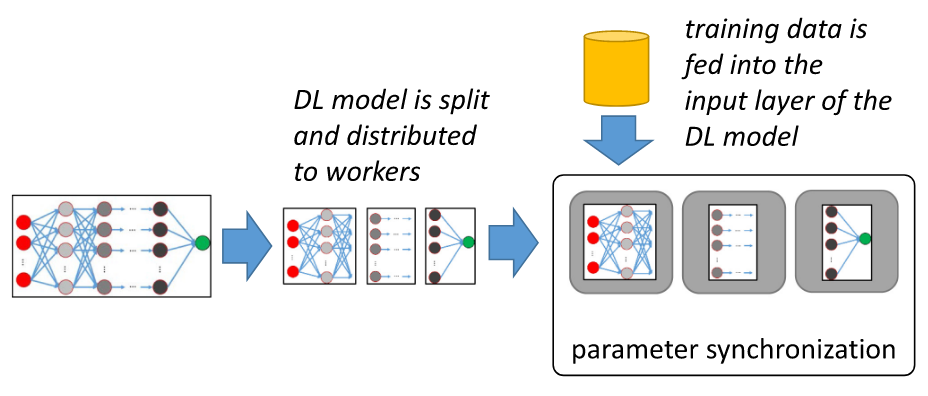
\includegraphics[width=\textwidth]{images/model parallelism.png} 
    \caption{Architecture Diagram of Model Parallelism  \cite{Mayer2020ScalableInfrastructures}}
    \label{fig:modelparallel}
  \end{center}
\end{figure}

The biggest challenge in model parallelism is to split the model into partitions that can be processed on different devices \cite{Mayer2017ThePath}. In many cases, the best way is to try out various permutations and measure the performance and keep the best permutation that has worked well. The second drawback is that model parallelism need heavy communication between devices. A combined effect of these two challenges is that stalling may occur if models are hard to be split effectively, to reduce the communication overloads and synchronization delays. Therefore, training speed might not increase linearly by increasing the number of parallel devices \cite{Mirhoseini2017DeviceLearning}.

The major benefit of the model parallelism is that it can accommodate huge deep learning networks, which cannot be stored on a single device (GPU) to train them because the memory required to train them is split to multiple devices. 

\subsubsection{Data Parallelism}
In data parallelism, copy the deep neural network into different devices and load an identical copy of the model on each device for training, as shown in Figure \ref{fig:dataparallel}. Split the data into the same number as the number of devices, and then data moves into the model replicas of the workers for training. Perform the training process on each chunk of the data that is assigned to the device, which leads to updates of the model parameters. Once it is completed on the devices, the parameters need to be synchronized across all the devices. 

\begin{figure}[ht]
  \begin{center}
    % below the size of the figure has been reduced for example
    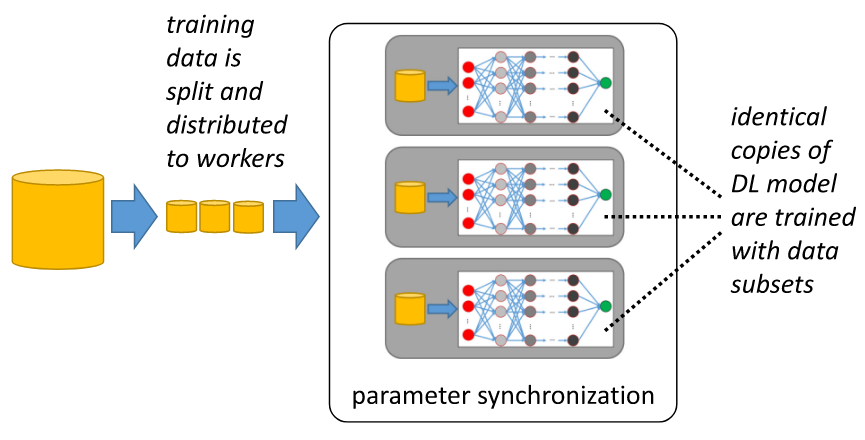
\includegraphics[width=\textwidth]{images/data parallelism.png} 
    \caption{Architecture Diagram of Data Parallelism  \cite{Mayer2020ScalableInfrastructures}}
    \label{fig:dataparallel}
  \end{center}
\end{figure}

Since on each device processes a mini batch of data, the total batch size is the product of the mini batch with the number of GPUs. This high data scale leads to poor convergence. The other drawback is that ideally, the data that is split along the different workers needs to be identically distributed, so that the parameter updates by the different workers can be easily synchronized to get the overall model \cite{Jia2018BeyondNetworks}.

The major benefit of data parallelism is that it can be easily applied to most of the deep learning networks without much specific knowledge about the architecture of the model. It is highly scalable for the cases when the training is compute intensive but have relatively few parameters like RNNs, CNNs \cite{Krizhevsky2014OneNetworks}.


\subsection{Types of synchronization}
Due to the multiple nodes trying to update the model, the important question then becomes when to synchronize the parameters between the parallel workers. The main trade off is between managing training convergence and quality with synchronization cost to update all the models on the parallel workers. There are mainly two methods which are discussed here: synchronous and asynchronous methods.

\subsubsection{Synchronous}
The workers synchronize the weight updates after every batch of data processed. This is implemented in some of the first and prominent methods, like the Bulk Synchronous Parallel (BSP) \cite{Valiant1990AComputation} method, which is already available in popular data analytics platforms. The main advantage is that the model convergence is easier due to the strict nature of synchronization. However, this method is vulnerable to a situation where \emph{one} single worker stalls the entire training process, especially when the different nodes in the system are heterogeneous in nature \cite{CiparSolvingStaleness}.

Synchronous training is already available in many open-source DL frameworks, such
as TensorFlow \cite{AbadiTensorFlow:Systems} and PyTorch \cite{Paszke2019PyTorch:Library}. Most ideally, it is best suited for a single node with multi GPUs where there are minimal delays from communication and due to the workers running on the same node, stragglers are not a significant issue.

\subsubsection{Asynchronous}
The workers update the model parameters completely independent of other workers. Asynchronous training relies on the theoretical characteristic of SGD that the model convergence is robust to the random ordering of data. The model used by a worker at some point of time might be a stale model because there are no binding guarantees. This makes it difficult to assess model convergence using asynchronous training. However, the advantage is that the workers enjoy great levels of flexibility during training, hence avoiding the straggler problem that is faced in the synchronous method.

\emph{Hogwild} \cite{NiuHOGWILD:Descent} is one implementation of the asynchronous training of parallel SGD. Hogwild works by providing all the workers access to a shared memory space, which consists of the model parameters. This is completely lock-free, and hence seems dangerous because new model parameters from one worker can be completely overwritten by another worker without being used at all. Nevertheless, their work show that since model updates are anyway random in nature when done sequentially, Hogwild also can achieve stellar performance. This has been applied to large neural networks with good results \cite{Deyringer2017ParallelizationHogwild}. 


\subsection{Data Parallel Systems Architecture}
The architecture of the system defines \emph{how} the parameter synchronization among different workers happens in a data parallel system. There are three major considerations for the system architecture. Firstly, the architecture must be able to scale up to many parallel workers to update the DL model and also read the updated DL model. Secondly, the system needs to be configurable, that is, to be able to manage different parameter settings, etc. The third aspect is to be compatible with widely available inter process communication primitives.

\begin{figure}[ht]
  \begin{center}
    % below the size of the figure has been reduced for example
    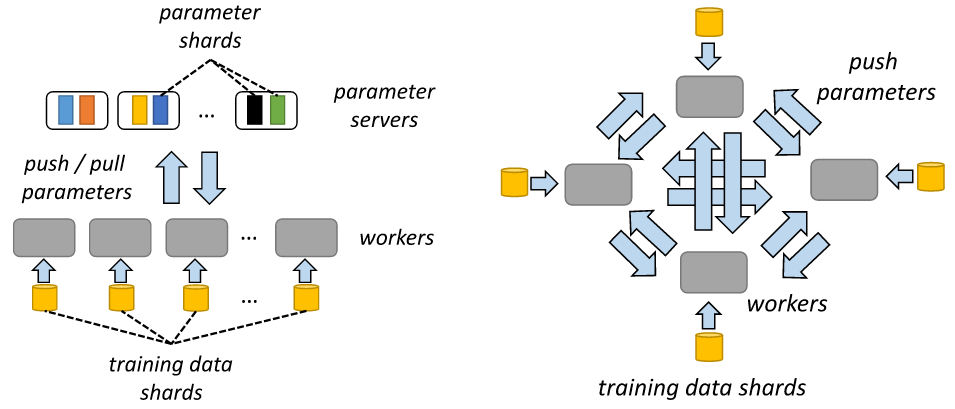
\includegraphics[width=\textwidth]{images/architecture_.png} 
    \caption{Diagram of Parameter Server architecture and Decentralised Architecture  \cite{Mayer2020ScalableInfrastructures}}
    \label{fig:arch}
  \end{center}
\end{figure}


\subsubsection{Centralized: Parameter Server}
Centralized architecture consists of a parameter server which is located (logically) in the centre and the worker nodes updates their computed gradients to the central server and all the workers then read the updated model to update their replicas of the model. This architecture is one of the most commonly used in a data parallel system. It is also common to use parameter shards to accelerate the process of communicating the parameter updates. Figure \ref{fig:arch} shows this architecture.

\subsubsection{Decentralized: \inlinecode{allreduce} Operation}
Decentralized architecture operates without a Parameter Server. The parameters synchronize directly by using an \inlinecode{allreduce} operation as shown in Figure \ref{fig:arch}. 

The major benefit of using a decentralized architecture is that there is no need for one node reserved for parameter server and the effort required to implement and maintain it. There is also no single point of failure, and this makes it easier to manage fault tolerance. The major drawback of the decentralized architecture is that communication increased exponentially with the increase in number of workers. One way to avoid this is to use partial gradient updates. For each synchronization, every worker sends a partition of the gradients to every other worker, this maybe be that it sends different partitions to different workers.  The communication costs now depend on the number of partitions \emph{and} also on the number of workers in the system. 

Both of these architectures, are widely adopted in leading open-source deep learning frameworks, however the decentralized architecture is the most suitable architecture for a system where there is a single node with multiple GPUs attached because communication on the same node does not cost much. However, for multinode training, a centralized architecture works better. 

A quick overview of practical considerations for different types of architecture, parallelism, and synchronization strategy can be accessed here \footnote{Distributed training with TensorFlow, TensorFlow Core. WebPage accessed on 22.8.2021. https://www.tensorflow.org/guide/distributed\_training}. 


\section{Related Large scale ASR}
Large-scale speech recognition has had varying definitions even over the past few years. In 2014, authors applied data and model parallelism for training RNN-based ASR models \cite{Hannun2014DeepRecognition}. They used 5000 hours of labelled data to build a multi-GPU powered data-driven speech system which produced state-of-the-art results for that period of time. This solution was also quite robust to distortions and designed to work on both clear, conversational speech and also speech in noisy environments. The work also showed that with data parallelism on more than a few GPUs, scaling up the overall batch size linearly with the number of GPUs did not help with the model convergence rate.

More recently, research works from large enterprise companies like Microsoft, Google focus on increasing the scale of training by multiple folds. Microsoft were the first to compare popular end to end speech recognition for large-scale ASR \cite{Li2020OnRecognition}. Authors consider an RNN transducer, an Attention-based encoder decoder, and transformer architectures and train them with 65,000 hours of training data both for streaming mode and non-streaming modes. In their experiments, to maintain a fair comparison, they have fixed the overall number of parameters to a single limit of around 87M. Their results show that transformer models obtained the best word error rates (WER) outperforming the other models by around 1\% WER. They also claim that pretraining works well even for large-scale tasks, compared to random initialization.

Google has also worked on increasing their scale of data used for their experiments. Authors have worked on building a domain invariant speech recognition model, using large amounts of data from multiple domains to train a single model that work across different applications, sampling rates, audio codecs and formats, and  encode decoder attention based model which can be used in multiple domains with  ease by retunoing it on a smaller data set of about 10 hours 
 
 
\section{Business Speech Dataset}

\subsection{Sharding}
\subsection{Sequential access}
\subsection{TAR advantages}
